\section{Results}
\label{sec:results}
\subsection{Landmark-specific prediction}
All 15 principal seed44 runs completed training and formal evaluation. The supplementary mean-pooling comparison contributed five additional completed runs. Every landmark evaluation contained the same 175 holdout patients and 56 positive labels. The aggregate results in Table~\ref{tab:main} were rebuilt from the saved prediction records and checked against the corresponding evaluation reports.
\begin{table}[t]
\centering
\caption{Seed44 performance on the fixed 175-patient internal holdout. Values are means of five separately evaluated fold models; AP denotes average precision and F1 uses a threshold of 0.5. Macro averages the three landmarks. These are not probability-ensemble scores.}
\label{tab:main}
\small
\begin{tabular}{llrrr}
\toprule
Model & Landmark & AUROC & AP & F1 \\
\midrule
NoJEPA & T0 & 0.7209 & 0.5749 & 0.5441 \\
NoJEPA & T1 & 0.7219 & 0.5815 & 0.5458 \\
NoJEPA & T2 & 0.7230 & 0.5812 & 0.5411 \\
NoJEPA & Macro & 0.7219 & 0.5792 & 0.5437 \\
\midrule
DirectReadout & T0 & 0.7304 & 0.5854 & 0.5447 \\
DirectReadout & T1 & 0.7306 & 0.5891 & 0.5485 \\
DirectReadout & T2 & 0.7299 & 0.5920 & 0.5685 \\
DirectReadout & Macro & 0.7303 & 0.5888 & 0.5539 \\
\midrule
ForecastAttention & T0 & 0.7294 & 0.5924 & 0.5334 \\
ForecastAttention & T1 & 0.7381 & 0.6012 & 0.5563 \\
ForecastAttention & T2 & 0.7421 & 0.6033 & 0.5510 \\
ForecastAttention & Macro & 0.7365 & 0.5990 & 0.5469 \\
\bottomrule
\end{tabular}
\end{table}


\fullmodel{} attained AUROCs of 0.7294, 0.7381, and 0.7421 at T0, T1, and T2, respectively. Relative to \nojepa{}, the absolute AUROC differences were +0.0084, +0.0162, and +0.0191. AP increased from 0.5924 at T0 to 0.6033 at T2. The three-landmark mean AUROC/AP/F1 was 0.7365/0.5990/0.5469, compared with 0.7219/0.5792/0.5437 for \nojepa{} and 0.7303/0.5888/0.5539 for \direct{}.

The full model did not lead every metric at every landmark. At T0, \direct{} had a slightly higher AUROC than \fullmodel{} (0.7304 versus 0.7294). \direct{} also had a higher T0 F1 (0.5447 versus 0.5334) and the highest T2 F1 (0.5685 versus 0.5510). Its three-landmark mean F1 exceeded that of \fullmodel{} by 0.0070. Thus the discrimination improvement of the forecast model did not translate into a uniform advantage at a fixed decision threshold.

\begin{figure}[t]
\centering
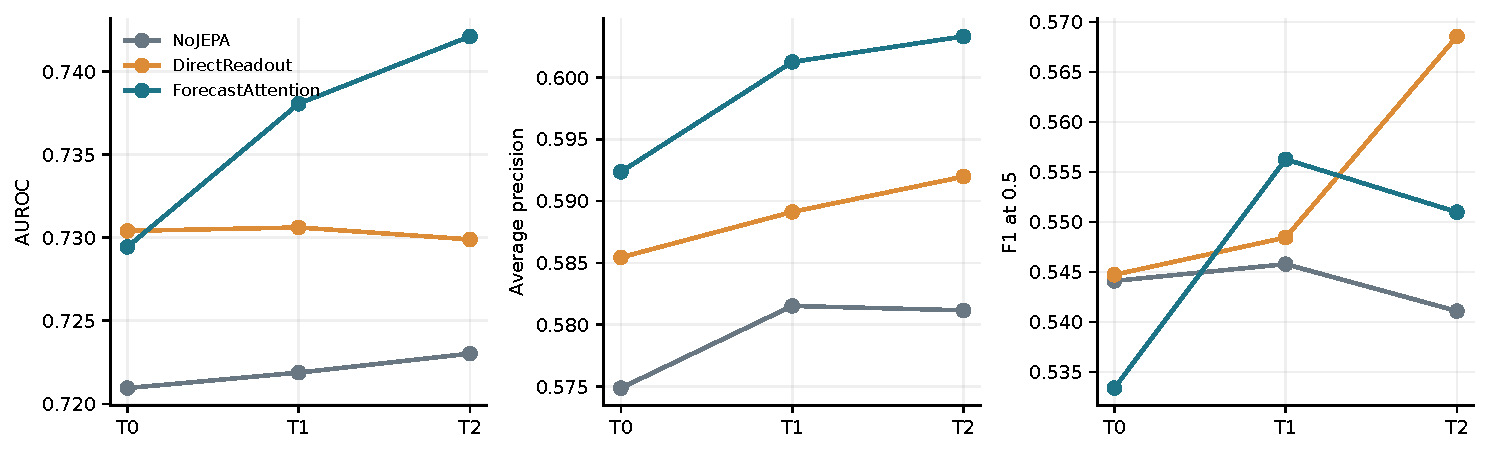
\includegraphics[width=\textwidth]{figures/landmark_performance.pdf}
\caption{Landmark-specific seed44 performance on the internal holdout. Each point averages metrics of five separately evaluated fold models. All landmarks use the same 175 patients. Lines connect landmark summaries and do not imply a statistically established temporal trend.}
\label{fig:landmarks}
\end{figure}

\subsection{Auxiliary supervision and forecast readout}
Adding future-state supervision while retaining direct readout increased mean AUROC by 0.0084, AP by 0.0097, and F1 by 0.0102 for \direct{} relative to \nojepa{}. Introducing the complete forecast-attention readout produced a further mean AUROC increase of 0.0062 and an AP increase of 0.0101 relative to \direct{}, accompanied by a mean F1 decrease of 0.0070. These two comparisons address different changes: the first isolates the auxiliary loss more closely, while the second changes both the classifier information pathway and its input representation.

The supplementary pooling comparison is provided in Table~\ref{tab:pooling}. Relative to \meanmodel{}, \fullmodel{} increased mean AUROC by 0.0017, AP by 0.0144, and F1 by 0.0011. At T0, however, its AUROC was lower by 0.0023 and its F1 was lower by 0.0113. The seed44 evidence therefore supports a modest descriptive aggregate difference between pooling choices, rather than a uniform attention advantage.

\subsection{Longitudinal change and calibration}
The observed T2--T0 AUROC difference was +0.0127 for \fullmodel{}, compared with +0.0021 for \nojepa{} and $-0.0005$ for \direct{}. The T1 value of \fullmodel{} lay between its T0 and T2 values. Because the same patients were evaluated at every landmark, these differences are not caused by changes in the evaluated patient set. They nevertheless reflect this trained configuration and do not establish that each individual's prediction improved or that added visits would be beneficial in another cohort.

Probability quality showed an unfavorable trade-off (Table~\ref{tab:calibration}). \fullmodel{} had higher mean NLL (0.6149), Brier score (0.2147), and ECE (0.1622) than \nojepa{} (0.5974, 0.2069, and 0.1310, respectively). Consequently, the AUROC and AP results should not be interpreted as improved calibrated risk estimation. No post-hoc calibration model was fitted in this analysis.
\begin{table}[t]
\centering
\caption{Calibration and probability accuracy, averaged over landmarks and five fold models for seed44. Lower is better. ECE uses ten equal-width bins.}
\label{tab:calibration}
\begin{tabular}{lrrr}
\toprule
Model & NLL & Brier & ECE \\
\midrule
NoJEPA & 0.5974 & 0.2069 & 0.1310 \\
DirectReadout & 0.5995 & 0.2073 & 0.1377 \\
ForecastAttention & 0.6149 & 0.2147 & 0.1622 \\
\bottomrule
\end{tabular}
\end{table}


\subsection{Conditional patient-level uncertainty}
The 95\% patient-bootstrap interval for mean AUROC was [0.6647, 0.8062] for \fullmodel{} and [0.6485, 0.7966] for \nojepa{}. The paired mean AUROC difference between these models was +0.0146, with interval [$-0.0062$, +0.0369]. The corresponding AP and F1 differences were +0.0198 [$-0.0161$, +0.0597] and +0.0032 [$-0.0339$, +0.0398]. Principal paired intervals included zero (Table~\ref{tab:bootstrap}), indicating that the observed differences remain uncertain even conditional on the fixed models. These intervals additionally omit the retrospective seed-selection uncertainty described in Section~\ref{sec:experiments}.
